% Created by tikzDevice version 0.12.6 on 2026-05-16 13:49:09
% !TEX encoding = UTF-8 Unicode
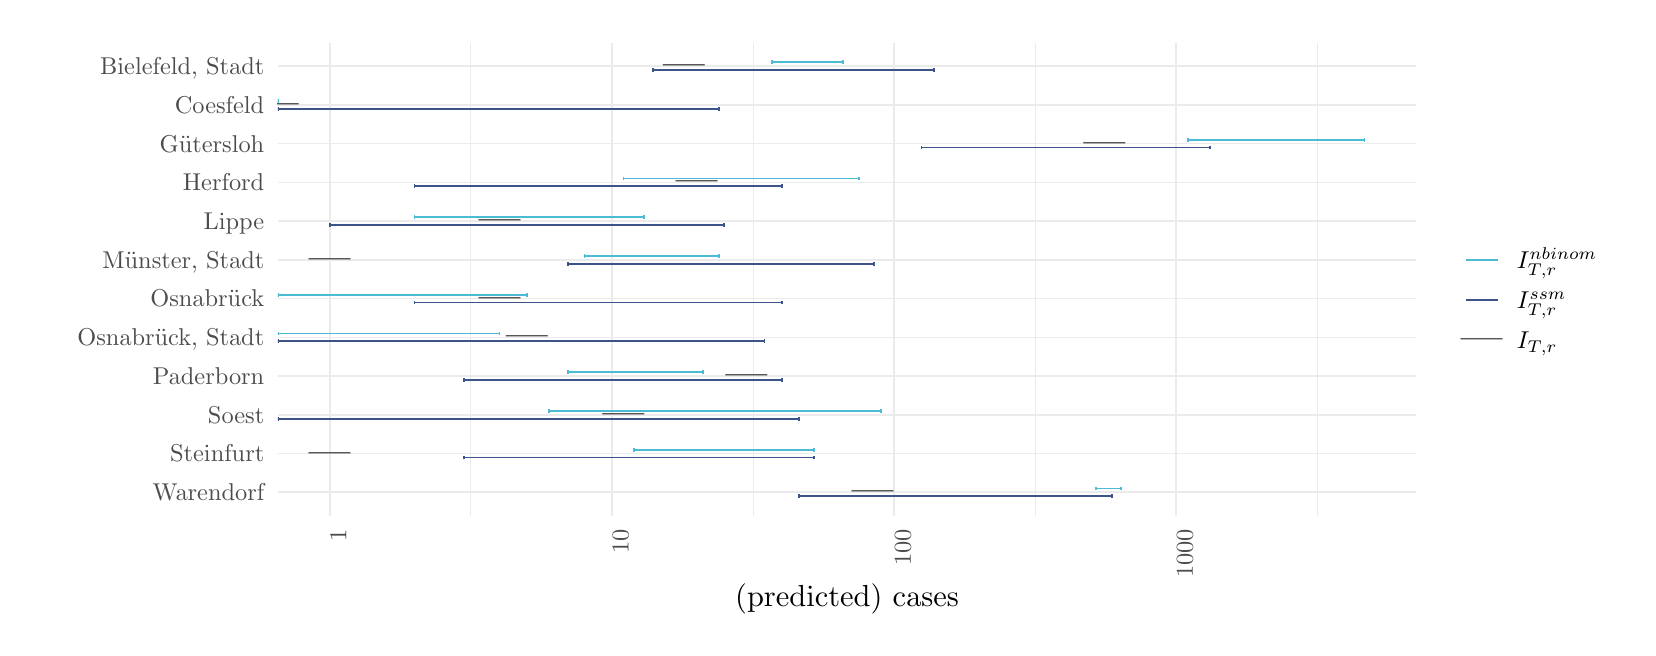
\begin{tikzpicture}[x=1pt,y=1pt]
\definecolor{fillColor}{RGB}{255,255,255}
\path[use as bounding box,fill=fillColor,fill opacity=0.00] (0,0) rectangle (578.16,216.81);
\begin{scope}
\path[clip] ( 90.44, 40.51) rectangle (501.70,211.31);
\definecolor{drawColor}{gray}{0.92}

\path[draw=drawColor,line width= 0.3pt,line join=round] (160.11, 40.51) --
	(160.11,211.31);

\path[draw=drawColor,line width= 0.3pt,line join=round] (262.07, 40.51) --
	(262.07,211.31);

\path[draw=drawColor,line width= 0.3pt,line join=round] (364.02, 40.51) --
	(364.02,211.31);

\path[draw=drawColor,line width= 0.3pt,line join=round] (465.98, 40.51) --
	(465.98,211.31);

\path[draw=drawColor,line width= 0.6pt,line join=round] ( 90.44, 48.91) --
	(501.70, 48.91);

\path[draw=drawColor,line width= 0.6pt,line join=round] ( 90.44, 62.91) --
	(501.70, 62.91);

\path[draw=drawColor,line width= 0.6pt,line join=round] ( 90.44, 76.91) --
	(501.70, 76.91);

\path[draw=drawColor,line width= 0.6pt,line join=round] ( 90.44, 90.91) --
	(501.70, 90.91);

\path[draw=drawColor,line width= 0.6pt,line join=round] ( 90.44,104.91) --
	(501.70,104.91);

\path[draw=drawColor,line width= 0.6pt,line join=round] ( 90.44,118.91) --
	(501.70,118.91);

\path[draw=drawColor,line width= 0.6pt,line join=round] ( 90.44,132.91) --
	(501.70,132.91);

\path[draw=drawColor,line width= 0.6pt,line join=round] ( 90.44,146.91) --
	(501.70,146.91);

\path[draw=drawColor,line width= 0.6pt,line join=round] ( 90.44,160.91) --
	(501.70,160.91);

\path[draw=drawColor,line width= 0.6pt,line join=round] ( 90.44,174.91) --
	(501.70,174.91);

\path[draw=drawColor,line width= 0.6pt,line join=round] ( 90.44,188.91) --
	(501.70,188.91);

\path[draw=drawColor,line width= 0.6pt,line join=round] ( 90.44,202.91) --
	(501.70,202.91);

\path[draw=drawColor,line width= 0.6pt,line join=round] (109.13, 40.51) --
	(109.13,211.31);

\path[draw=drawColor,line width= 0.6pt,line join=round] (211.09, 40.51) --
	(211.09,211.31);

\path[draw=drawColor,line width= 0.6pt,line join=round] (313.04, 40.51) --
	(313.04,211.31);

\path[draw=drawColor,line width= 0.6pt,line join=round] (415.00, 40.51) --
	(415.00,211.31);
\definecolor{drawColor}{RGB}{0,0,0}

\node[text=drawColor,anchor=base,inner sep=0pt, outer sep=0pt, scale=  1.52] at (180.40,101.12) {|};

\node[text=drawColor,anchor=base,inner sep=0pt, outer sep=0pt, scale=  1.52] at (170.52,115.12) {|};

\node[text=drawColor,anchor=base,inner sep=0pt, outer sep=0pt, scale=  1.52] at (109.13,129.12) {|};

\node[text=drawColor,anchor=base,inner sep=0pt, outer sep=0pt, scale=  1.52] at ( 90.44,185.12) {|};

\node[text=drawColor,anchor=base,inner sep=0pt, outer sep=0pt, scale=  1.52] at (109.13, 59.12) {|};

\node[text=drawColor,anchor=base,inner sep=0pt, outer sep=0pt, scale=  1.52] at (305.32, 45.12) {|};

\node[text=drawColor,anchor=base,inner sep=0pt, outer sep=0pt, scale=  1.52] at (237.11,199.12) {|};

\node[text=drawColor,anchor=base,inner sep=0pt, outer sep=0pt, scale=  1.52] at (389.09,171.12) {|};

\node[text=drawColor,anchor=base,inner sep=0pt, outer sep=0pt, scale=  1.52] at (241.78,157.12) {|};

\node[text=drawColor,anchor=base,inner sep=0pt, outer sep=0pt, scale=  1.52] at (170.52,143.12) {|};

\node[text=drawColor,anchor=base,inner sep=0pt, outer sep=0pt, scale=  1.52] at (259.73, 87.12) {|};

\node[text=drawColor,anchor=base,inner sep=0pt, outer sep=0pt, scale=  1.52] at (215.31, 73.12) {|};
\definecolor{drawColor}{RGB}{77,187,213}

\path[draw=drawColor,line width= 0.6pt,line join=round] (170.52,105.61) --
	(170.52,107.01);

\path[draw=drawColor,line width= 0.6pt,line join=round] (170.52,106.31) --
	( 90.44,106.31);

\path[draw=drawColor,line width= 0.6pt,line join=round] ( 90.44,105.61) --
	( 90.44,107.01);

\path[draw=drawColor,line width= 0.6pt,line join=round] (180.40,119.61) --
	(180.40,121.01);

\path[draw=drawColor,line width= 0.6pt,line join=round] (180.40,120.31) --
	( 90.44,120.31);

\path[draw=drawColor,line width= 0.6pt,line join=round] ( 90.44,119.61) --
	( 90.44,121.01);

\path[draw=drawColor,line width= 0.6pt,line join=round] (249.85,133.61) --
	(249.85,135.01);

\path[draw=drawColor,line width= 0.6pt,line join=round] (249.85,134.31) --
	(201.21,134.31);

\path[draw=drawColor,line width= 0.6pt,line join=round] (201.21,133.61) --
	(201.21,135.01);

\path[draw=drawColor,line width= 0.6pt,line join=round] ( 90.44,189.61) --
	( 90.44,191.01);

\path[draw=drawColor,line width= 0.6pt,line join=round] ( 90.44,190.31) --
	( 90.44,190.31);

\path[draw=drawColor,line width= 0.6pt,line join=round] ( 90.44,189.61) --
	( 90.44,191.01);

\path[draw=drawColor,line width= 0.6pt,line join=round] (284.09, 63.61) --
	(284.09, 65.01);

\path[draw=drawColor,line width= 0.6pt,line join=round] (284.09, 64.31) --
	(219.16, 64.31);

\path[draw=drawColor,line width= 0.6pt,line join=round] (219.16, 63.61) --
	(219.16, 65.01);

\path[draw=drawColor,line width= 0.6pt,line join=round] (395.17, 49.61) --
	(395.17, 51.01);

\path[draw=drawColor,line width= 0.6pt,line join=round] (395.17, 50.31) --
	(386.13, 50.31);

\path[draw=drawColor,line width= 0.6pt,line join=round] (386.13, 49.61) --
	(386.13, 51.01);

\path[draw=drawColor,line width= 0.6pt,line join=round] (294.64,203.61) --
	(294.64,205.01);

\path[draw=drawColor,line width= 0.6pt,line join=round] (294.64,204.31) --
	(269.02,204.31);

\path[draw=drawColor,line width= 0.6pt,line join=round] (269.02,203.61) --
	(269.02,205.01);

\path[draw=drawColor,line width= 0.6pt,line join=round] (483.01,175.61) --
	(483.01,177.01);

\path[draw=drawColor,line width= 0.6pt,line join=round] (483.01,176.31) --
	(419.18,176.31);

\path[draw=drawColor,line width= 0.6pt,line join=round] (419.18,175.61) --
	(419.18,177.01);

\path[draw=drawColor,line width= 0.6pt,line join=round] (300.30,161.61) --
	(300.30,163.01);

\path[draw=drawColor,line width= 0.6pt,line join=round] (300.30,162.31) --
	(215.31,162.31);

\path[draw=drawColor,line width= 0.6pt,line join=round] (215.31,161.61) --
	(215.31,163.01);

\path[draw=drawColor,line width= 0.6pt,line join=round] (222.70,147.61) --
	(222.70,149.01);

\path[draw=drawColor,line width= 0.6pt,line join=round] (222.70,148.31) --
	(139.82,148.31);

\path[draw=drawColor,line width= 0.6pt,line join=round] (139.82,147.61) --
	(139.82,149.01);

\path[draw=drawColor,line width= 0.6pt,line join=round] (243.94, 91.61) --
	(243.94, 93.01);

\path[draw=drawColor,line width= 0.6pt,line join=round] (243.94, 92.31) --
	(195.29, 92.31);

\path[draw=drawColor,line width= 0.6pt,line join=round] (195.29, 91.61) --
	(195.29, 93.01);

\path[draw=drawColor,line width= 0.6pt,line join=round] (308.38, 77.61) --
	(308.38, 79.01);

\path[draw=drawColor,line width= 0.6pt,line join=round] (308.38, 78.31) --
	(188.47, 78.31);

\path[draw=drawColor,line width= 0.6pt,line join=round] (188.47, 77.61) --
	(188.47, 79.01);
\definecolor{drawColor}{RGB}{60,84,136}

\path[draw=drawColor,line width= 0.6pt,line join=round] (266.29,102.81) --
	(266.29,104.21);

\path[draw=drawColor,line width= 0.6pt,line join=round] (266.29,103.51) --
	( 90.44,103.51);

\path[draw=drawColor,line width= 0.6pt,line join=round] ( 90.44,102.81) --
	( 90.44,104.21);

\path[draw=drawColor,line width= 0.6pt,line join=round] (272.47,116.81) --
	(272.47,118.21);

\path[draw=drawColor,line width= 0.6pt,line join=round] (272.47,117.51) --
	(139.82,117.51);

\path[draw=drawColor,line width= 0.6pt,line join=round] (139.82,116.81) --
	(139.82,118.21);

\path[draw=drawColor,line width= 0.6pt,line join=round] (305.75,130.81) --
	(305.75,132.21);

\path[draw=drawColor,line width= 0.6pt,line join=round] (305.75,131.51) --
	(195.29,131.51);

\path[draw=drawColor,line width= 0.6pt,line join=round] (195.29,130.81) --
	(195.29,132.21);

\path[draw=drawColor,line width= 0.6pt,line join=round] (249.85,186.81) --
	(249.85,188.21);

\path[draw=drawColor,line width= 0.6pt,line join=round] (249.85,187.51) --
	( 90.44,187.51);

\path[draw=drawColor,line width= 0.6pt,line join=round] ( 90.44,186.81) --
	( 90.44,188.21);

\path[draw=drawColor,line width= 0.6pt,line join=round] (284.09, 60.81) --
	(284.09, 62.21);

\path[draw=drawColor,line width= 0.6pt,line join=round] (284.09, 61.51) --
	(157.78, 61.51);

\path[draw=drawColor,line width= 0.6pt,line join=round] (157.78, 60.81) --
	(157.78, 62.21);

\path[draw=drawColor,line width= 0.6pt,line join=round] (391.91, 46.81) --
	(391.91, 48.21);

\path[draw=drawColor,line width= 0.6pt,line join=round] (391.91, 47.51) --
	(278.66, 47.51);

\path[draw=drawColor,line width= 0.6pt,line join=round] (278.66, 46.81) --
	(278.66, 48.21);

\path[draw=drawColor,line width= 0.6pt,line join=round] (327.61,200.81) --
	(327.61,202.21);

\path[draw=drawColor,line width= 0.6pt,line join=round] (327.61,201.51) --
	(225.99,201.51);

\path[draw=drawColor,line width= 0.6pt,line join=round] (225.99,200.81) --
	(225.99,202.21);

\path[draw=drawColor,line width= 0.6pt,line join=round] (427.17,172.81) --
	(427.17,174.21);

\path[draw=drawColor,line width= 0.6pt,line join=round] (427.17,173.51) --
	(322.92,173.51);

\path[draw=drawColor,line width= 0.6pt,line join=round] (322.92,172.81) --
	(322.92,174.21);

\path[draw=drawColor,line width= 0.6pt,line join=round] (272.47,158.81) --
	(272.47,160.21);

\path[draw=drawColor,line width= 0.6pt,line join=round] (272.47,159.51) --
	(139.82,159.51);

\path[draw=drawColor,line width= 0.6pt,line join=round] (139.82,158.81) --
	(139.82,160.21);

\path[draw=drawColor,line width= 0.6pt,line join=round] (251.66,144.81) --
	(251.66,146.21);

\path[draw=drawColor,line width= 0.6pt,line join=round] (251.66,145.51) --
	(109.13,145.51);

\path[draw=drawColor,line width= 0.6pt,line join=round] (109.13,144.81) --
	(109.13,146.21);

\path[draw=drawColor,line width= 0.6pt,line join=round] (272.47, 88.81) --
	(272.47, 90.21);

\path[draw=drawColor,line width= 0.6pt,line join=round] (272.47, 89.51) --
	(157.78, 89.51);

\path[draw=drawColor,line width= 0.6pt,line join=round] (157.78, 88.81) --
	(157.78, 90.21);

\path[draw=drawColor,line width= 0.6pt,line join=round] (278.66, 74.81) --
	(278.66, 76.21);

\path[draw=drawColor,line width= 0.6pt,line join=round] (278.66, 75.51) --
	( 90.44, 75.51);

\path[draw=drawColor,line width= 0.6pt,line join=round] ( 90.44, 74.81) --
	( 90.44, 76.21);
\end{scope}
\begin{scope}
\path[clip] (  0.00,  0.00) rectangle (578.16,216.81);
\definecolor{drawColor}{gray}{0.30}

\node[text=drawColor,anchor=base east,inner sep=0pt, outer sep=0pt, scale=  0.88] at ( 85.49, 45.88) {Warendorf};

\node[text=drawColor,anchor=base east,inner sep=0pt, outer sep=0pt, scale=  0.88] at ( 85.49, 59.88) {Steinfurt};

\node[text=drawColor,anchor=base east,inner sep=0pt, outer sep=0pt, scale=  0.88] at ( 85.49, 73.88) {Soest};

\node[text=drawColor,anchor=base east,inner sep=0pt, outer sep=0pt, scale=  0.88] at ( 85.49, 87.88) {Paderborn};

\node[text=drawColor,anchor=base east,inner sep=0pt, outer sep=0pt, scale=  0.88] at ( 85.49,101.88) {Osnabrück, Stadt};

\node[text=drawColor,anchor=base east,inner sep=0pt, outer sep=0pt, scale=  0.88] at ( 85.49,115.88) {Osnabrück};

\node[text=drawColor,anchor=base east,inner sep=0pt, outer sep=0pt, scale=  0.88] at ( 85.49,129.88) {Münster, Stadt};

\node[text=drawColor,anchor=base east,inner sep=0pt, outer sep=0pt, scale=  0.88] at ( 85.49,143.88) {Lippe};

\node[text=drawColor,anchor=base east,inner sep=0pt, outer sep=0pt, scale=  0.88] at ( 85.49,157.88) {Herford};

\node[text=drawColor,anchor=base east,inner sep=0pt, outer sep=0pt, scale=  0.88] at ( 85.49,171.88) {Gütersloh};

\node[text=drawColor,anchor=base east,inner sep=0pt, outer sep=0pt, scale=  0.88] at ( 85.49,185.88) {Coesfeld};

\node[text=drawColor,anchor=base east,inner sep=0pt, outer sep=0pt, scale=  0.88] at ( 85.49,199.88) {Bielefeld, Stadt};
\end{scope}
\begin{scope}
\path[clip] (  0.00,  0.00) rectangle (578.16,216.81);
\definecolor{drawColor}{gray}{0.30}

\node[text=drawColor,rotate= 90.00,anchor=base east,inner sep=0pt, outer sep=0pt, scale=  0.88] at (115.19, 35.56) {1};

\node[text=drawColor,rotate= 90.00,anchor=base east,inner sep=0pt, outer sep=0pt, scale=  0.88] at (217.15, 35.56) {10};

\node[text=drawColor,rotate= 90.00,anchor=base east,inner sep=0pt, outer sep=0pt, scale=  0.88] at (319.10, 35.56) {100};

\node[text=drawColor,rotate= 90.00,anchor=base east,inner sep=0pt, outer sep=0pt, scale=  0.88] at (421.06, 35.56) {1000};
\end{scope}
\begin{scope}
\path[clip] (  0.00,  0.00) rectangle (578.16,216.81);
\definecolor{drawColor}{RGB}{0,0,0}

\node[text=drawColor,anchor=base,inner sep=0pt, outer sep=0pt, scale=  1.10] at (296.07,  7.64) {(predicted) cases};
\end{scope}
\begin{scope}
\path[clip] (  0.00,  0.00) rectangle (578.16,216.81);
\definecolor{drawColor}{RGB}{77,187,213}

\path[draw=drawColor,line width= 0.6pt,line join=round] (519.65,132.76) -- (531.21,132.76);
\end{scope}
\begin{scope}
\path[clip] (  0.00,  0.00) rectangle (578.16,216.81);
\definecolor{drawColor}{RGB}{60,84,136}

\path[draw=drawColor,line width= 0.6pt,line join=round] (519.65,118.30) -- (531.21,118.30);
\end{scope}
\begin{scope}
\path[clip] (  0.00,  0.00) rectangle (578.16,216.81);
\definecolor{drawColor}{RGB}{0,0,0}

\node[text=drawColor,anchor=base,inner sep=0pt, outer sep=0pt, scale=  1.52] at (525.43,100.06) {|};
\end{scope}
\begin{scope}
\path[clip] (  0.00,  0.00) rectangle (578.16,216.81);
\definecolor{drawColor}{RGB}{0,0,0}

\node[text=drawColor,anchor=base west,inner sep=0pt, outer sep=0pt, scale=  0.88] at (538.16,129.73) {$I^{nbinom}_{T, r}$};
\end{scope}
\begin{scope}
\path[clip] (  0.00,  0.00) rectangle (578.16,216.81);
\definecolor{drawColor}{RGB}{0,0,0}

\node[text=drawColor,anchor=base west,inner sep=0pt, outer sep=0pt, scale=  0.88] at (538.16,115.27) {$I^{ssm}_{T, r}$};
\end{scope}
\begin{scope}
\path[clip] (  0.00,  0.00) rectangle (578.16,216.81);
\definecolor{drawColor}{RGB}{0,0,0}

\node[text=drawColor,anchor=base west,inner sep=0pt, outer sep=0pt, scale=  0.88] at (538.16,100.82) {$I_{T, r}$};
\end{scope}
\end{tikzpicture}
